\begin{thm}{185}{\hosi 9}{東京大 後期 (2005) 誘導抜き}
 $a$は実数で、$\dfrac{1}{2}\le a\le 2$ を満たすとする。$xy$平面の領域$D, E$を、
 \begin{align*}
  D:&\quad 1\le x^2+y^2 \le 4 \\
  E:&\quad a\le x \le a+1
 \end{align*}
 で定める。領域$D$と$E$の共通部分の面積を$a$の関数と考えて$S(a)$とおく。$S(a)$を最大にするような$a$の値を求めよ。
\end{thm}

\begin{figure}[H]
 \centering
 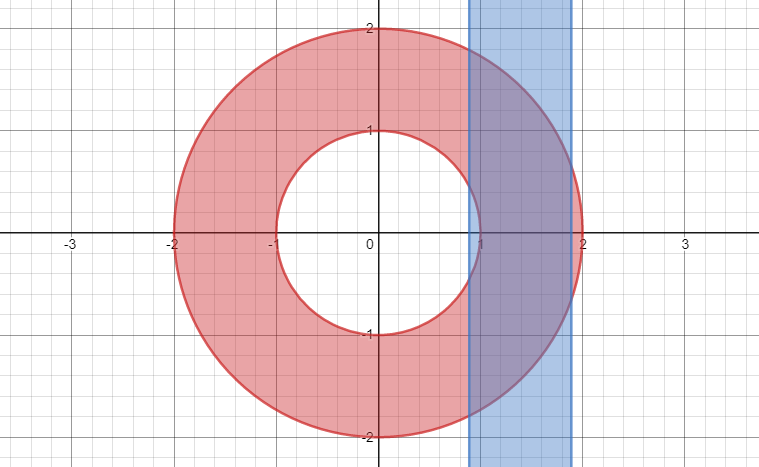
\includegraphics[width=0.8\linewidth]{../problems/Q_185/A_185.png}
\end{figure}

$S(a)$は次のように求められる。
\begin{align*}
 S(a)=\left\{
 \begin{aligned}
  &2\int_a^{a+1}\!\!\!\sqrt{4-x^2} \,dx - 2\int_a^1\!\!\sqrt{1-x^2} \,dx & &(\frac{1}{2}\le a\le 1) \\
  &2\int_a^2\!\!\sqrt{4-x^2} \,dx & &(1\le a\le 2)
  \end{aligned}
  \right.
\end{align*}
$1\le a\le 2$の範囲では$S(a)$は明らかに単調減少となるから、$S(a)$を最大にするような$a$は$\dfrac12\le a\le 1$の範囲に存在する。以降$a$は$\dfrac12\le a\le 1$の範囲で考える。微分すると、
\begin{align*}
 S'(a) &= 2\left(\sqrt{4-(a+1)^2}-\sqrt{4-a^2}+\sqrt{1-a^2}\right)
\end{align*}
を得る。これについて、
\begin{align*}
 S'\left(\frac{1}{2}\right)&=\frac{\sqrt{17}-\sqrt{15}+\sqrt{3}}{2} > 0 \\
 S'(1)&=-\sqrt{3} < 0
\end{align*}
となる。2階微分は、
\begin{align*}
 S''(a)=-\frac{-(a+1)}{\sqrt{4-(a+1)^2}}-a\left(\frac{1}{\sqrt{1-a^2}}-\frac{1}{\sqrt{4-a^2}}\right)
\end{align*}
である。$\dfrac{1}{2}\le a\le 1$において、$4-a^2>1-a^2>0$が成り立っていることに注意すると、この範囲においては常に$S''(a)<0$である。したがって、$S'(a)$は単調減少し、$S'\left(\dfrac{1}{2}\right)>0$ と$S'(1)<0$であることから、$\dfrac{1}{2}<c<1$なる実数$c$がただ一つ存在して、$S'(c)=0$を満たし、$S(c)$が極大となることがわかる。

方程式$S'(a)=0$を$\dfrac{1}{2}<a<1$のもとで解く。
\[ 4-(a+1)^2=(1-a)(3+a) \]
となることに注意して、
\begin{align*}
 \sqrt{1-a}\left[\sqrt{3+a}+\sqrt{1+a}\right]&=\sqrt{4-a^2} \\
 \dou\quad 2(1-a)\left[(2+a)+\sqrt{(3+a)(1+a)}\right]&=(2-a)(2+a) \\
 \dou\quad 2(1-a)\sqrt{(3+a)(1+a)}&=a(2+a) \\
 \dou\quad 4(1-a)^2(3+a)(1+a)&=a^2(2+a)^2 \\
 \dou\quad 3a^4+4a^3-20a^2-8a+12&=0
\end{align*}
と整理できる。ここで$a=0$は明らかに解でないから両辺$a^2$で割って、
\begin{align*}
 3a^2+4a-20-8\frac{1}{a}+12\frac{1}{a^2}&=0 \\
 3\left(a^2+\frac{4}{a^2}\right)+4\left(a-\frac{2}{a}\right)-20&=0 \\
 3(t^2+4)+4t-20&=0 \\
 \therefore\quad t&=\frac{-2\pm2\sqrt{7}}{3}
\end{align*}
となる。なお、$t=a-\dfrac{2}{a}$ とした。$\dfrac{1}{2}<a<1$のもとでは$-\dfrac{7}{2}<t<-1$なので、符号は負のみが適する。最後に$a$について解けば、
\begin{align*}
 a^2-ta-2&=0 \\
 \therefore\quad a&=\frac{t\pm\sqrt{t^2+8}}{2}
\end{align*}
$\dfrac{1}{2}<a<1$より符号は正のみ適する。$t=\dfrac{-2-2\sqrt{7}}{3}$を用いて整理すれば、求める$a$の値は
\[ a=\frac{1}{3}\left(-1-\sqrt{7}+\sqrt{26+2\sqrt{7}}\right) \]